\begin{center}
    {\LARGE \textbf{2014有机化学}} \\[2ex]
    {\large 时量180分钟 \quad 满分150分}
\end{center}

\vspace{0.5cm}
\noindent\textbf{注意事项:}
\begin{enumerate}[label=\arabic*., parsep=0pt, itemsep=0pt]
    \item 答题前,考生先将自己的姓名、学号、考场号、座位号填写在答题卡上,将条形码准确粘贴在考生信息条形码粘贴区。
    \item 考试结束后,将本试卷与答题纸一并收回。
    \item 回答各个问题时,将答案写在答题纸上,写在本试卷上无效。
\end{enumerate}

\vspace{0.5cm}
\noindent\textbf{一、完成反应(30 pts.)}

\begin{enumerate}[label=\arabic*., itemsep=3ex]
    \item 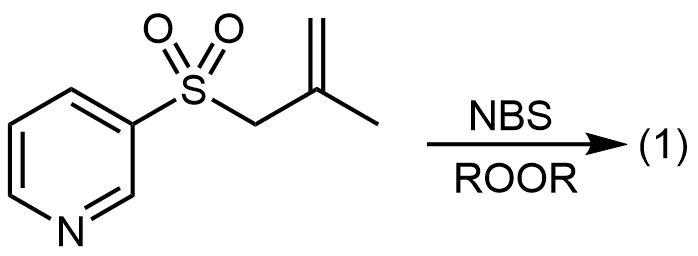
\includegraphics[scale=0.3, valign=c]{./Figure/2014/2014_1_1.png} 
    \item 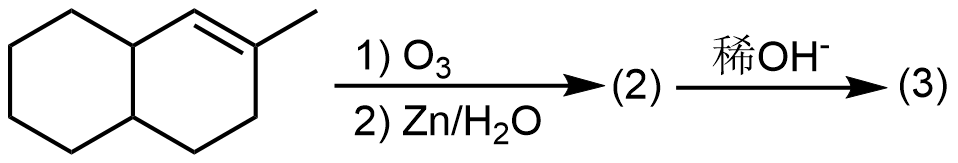
\includegraphics[scale=0.3, valign=c]{./Figure/2014/2014_1_2.png}
    \item 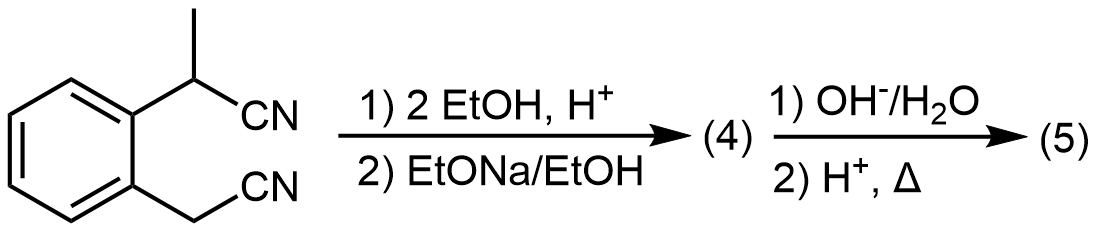
\includegraphics[scale=0.3, valign=c]{./Figure/2014/2014_1_3.png}
    \item 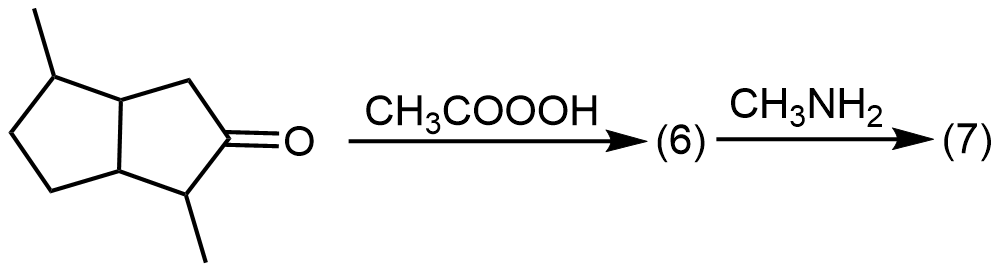
\includegraphics[scale=0.3, valign=c]{./Figure/2014/2014_1_4.png}
    \item 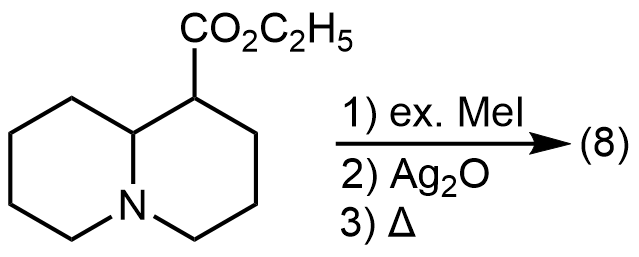
\includegraphics[scale=0.3, valign=c]{./Figure/2014/2014_1_5.png}
    \item 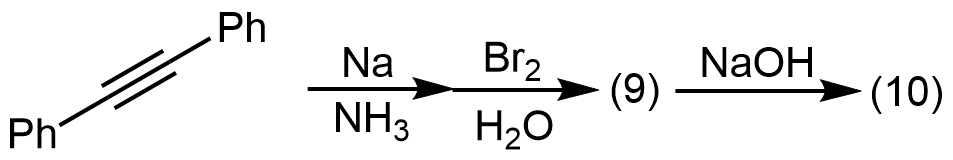
\includegraphics[scale=0.3, valign=c]{./Figure/2014/2014_1_6.png}
    \item 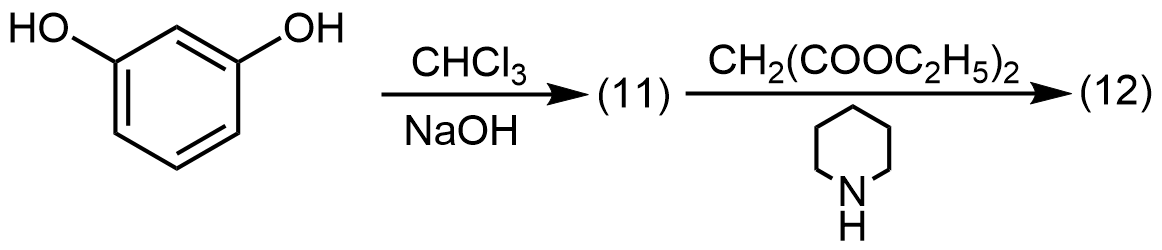
\includegraphics[scale=0.3, valign=c]{./Figure/2014/2014_1_7.png}
    \item 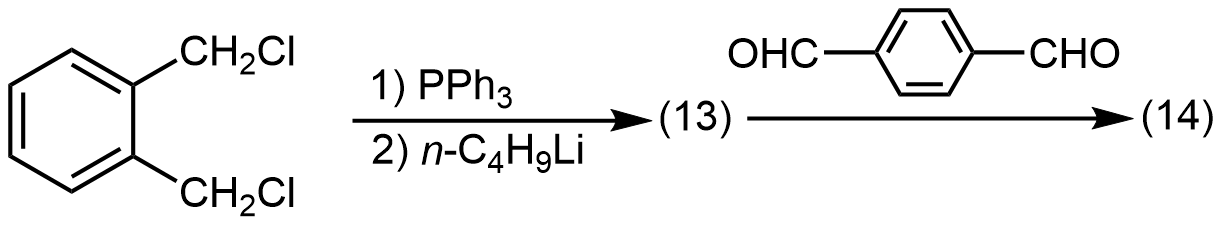
\includegraphics[scale=0.3, valign=c]{./Figure/2014/2014_1_8.png}
    \item 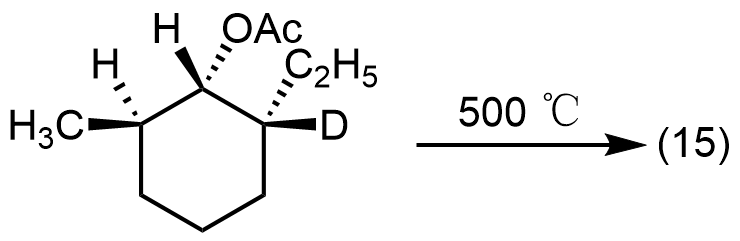
\includegraphics[scale=0.3, valign=c]{./Figure/2014/2014_1_9.png}

\end{enumerate}

\vspace{0.5cm}
\noindent\textbf{二、机理题(30 pts.)}

\begin{enumerate}[label=\arabic*., start=1, itemsep=1.5ex]
    \item 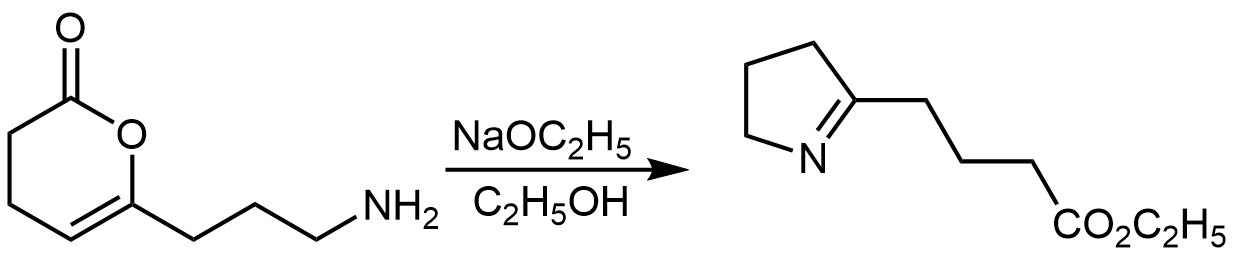
\includegraphics[scale=0.3, valign=c]{./Figure/2014/2014_2_1.png}
    \item 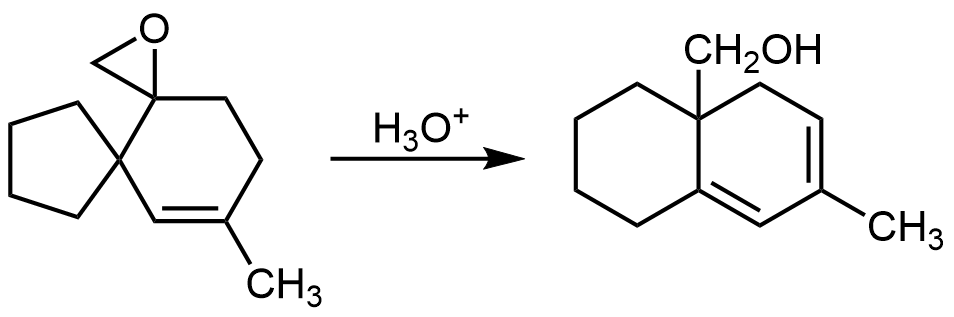
\includegraphics[scale=0.3, valign=c]{./Figure/2014/2014_2_2.png}
    \item 无论是(Z)-2-苯基-2-丁烯还是(E)-2-苯基-2-丁烯在ROOR存在下与HBr反应，均生成外消旋的2-溴-3-苯基丁烷，从活性中间体构象的角度说明该反应为什么没有立体选择性？
\end{enumerate}

\vspace{0.5cm}
\noindent\textbf{三、合成题(30 pts.)}

\begin{enumerate}[label=\arabic*., start=1, itemsep=1.5ex]

    \begin{figure}[htbp]
        \centering
        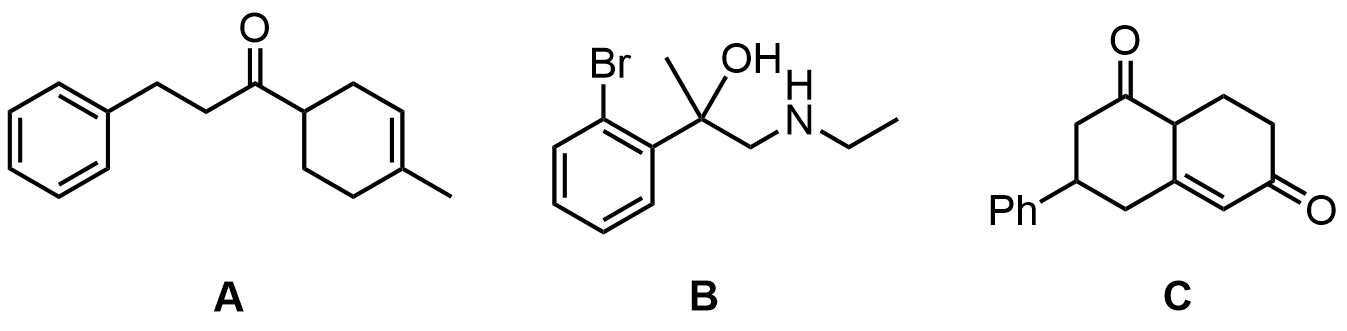
\includegraphics[scale=0.3]{./Figure/2014/2014_3.png}
    \end{figure}
    \item 以苯、小于等于3个碳的有机物合成\textbf{A}
    \item 以苯、小于等于3个碳的有机物合成\textbf{B}
    \item 以苯、小于等于3个碳的有机物合成\textbf{C}
\end{enumerate}

\vspace{0.5cm}
\noindent\textbf{四、综合题(30 pts.)}

\begin{center}
    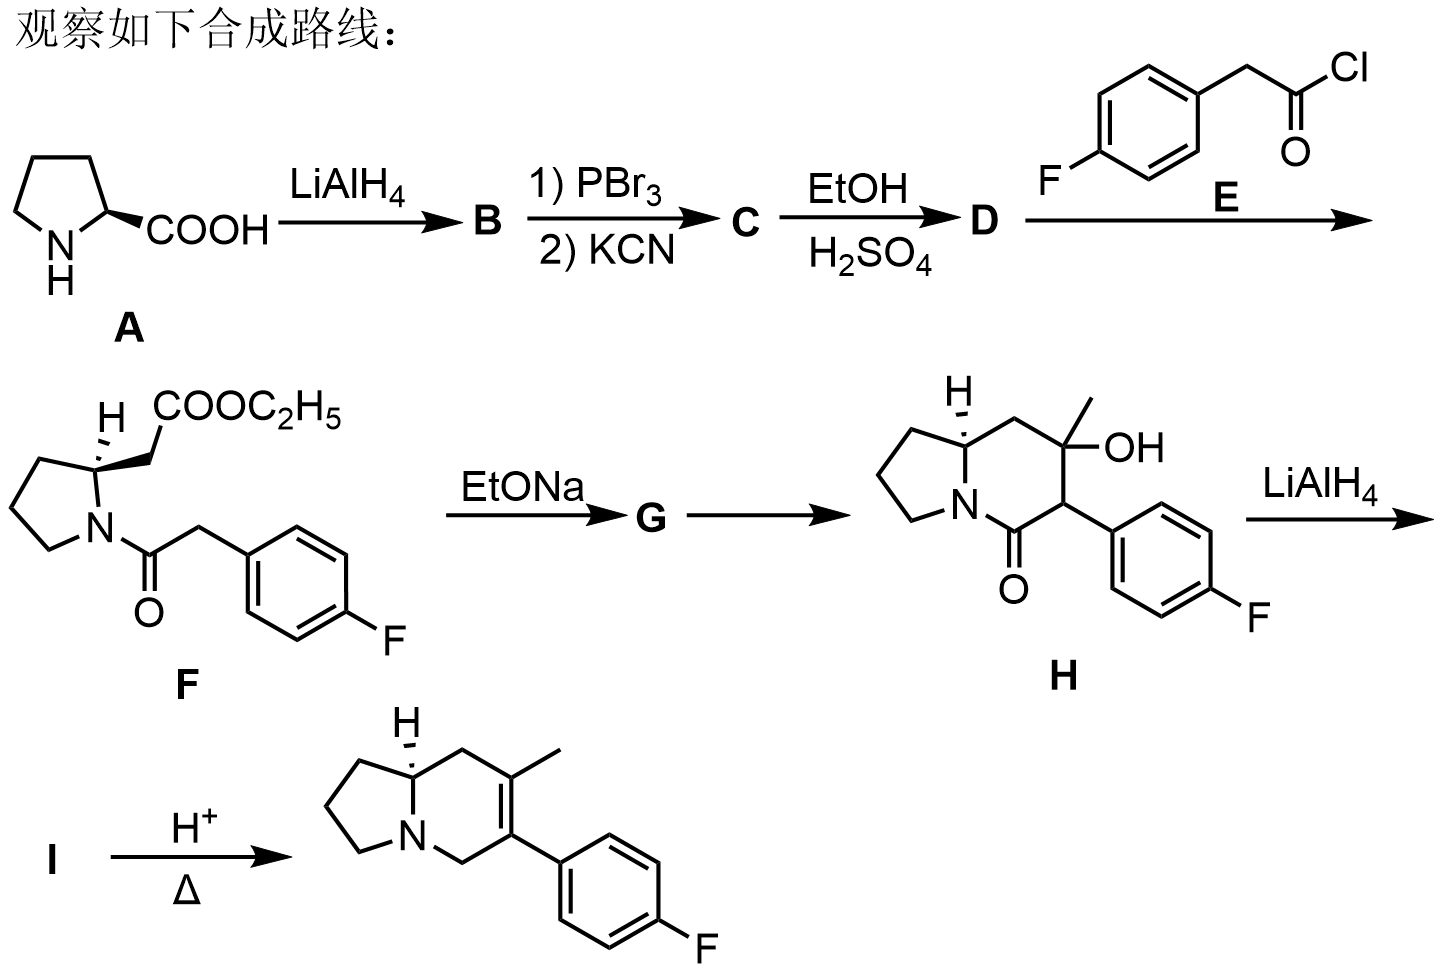
\includegraphics[scale=0.3]{./Figure/2014/2014_4.png}
\end{center}

\begin{enumerate}[label=\arabic*., itemsep=1.2ex]
    \item 写出化合物B、C、D、G、I的结构式。(10 pts.)
    \item 写出化合物F转化成化合物G的反应机理。(6 pts.)
    \item 写出化合物G转化成化合物H的反应条件。(3 pts.)
    \item 以乙酰氨基丙二酸二乙酯和小于等于3个碳的有机物与必要的无机试剂合成外消旋的脯氨酸（外消旋的化合物A）。(4 pts.)
    \item 以苯与小于等于3个碳的有机物与必要的无机试剂合成化合物E。(7 pts.)
\end{enumerate}

\vspace{0.5cm}
\noindent\textbf{五、实验题 略}